% !TEX program = xelatex

\documentclass[hidelinks, 12pt, a4paper]{article}

\usepackage{fontspec}
\setmainfont[Ligatures=TeX]{Linux Libertine O}

\usepackage[hidelinks, colorlinks = true, urlcolor = blue]{hyperref}

\usepackage{indentfirst}
\usepackage{graphicx}
\usepackage[left=2cm,right=2cm,top=2cm,bottom=2cm]{geometry}
\usepackage{lipsum}

%\setlength{\parindent}{1em}
%\setlength{\parskip}{1em}\title{Εργασία Στατιστικής}

%\title{Java socket programming \\ 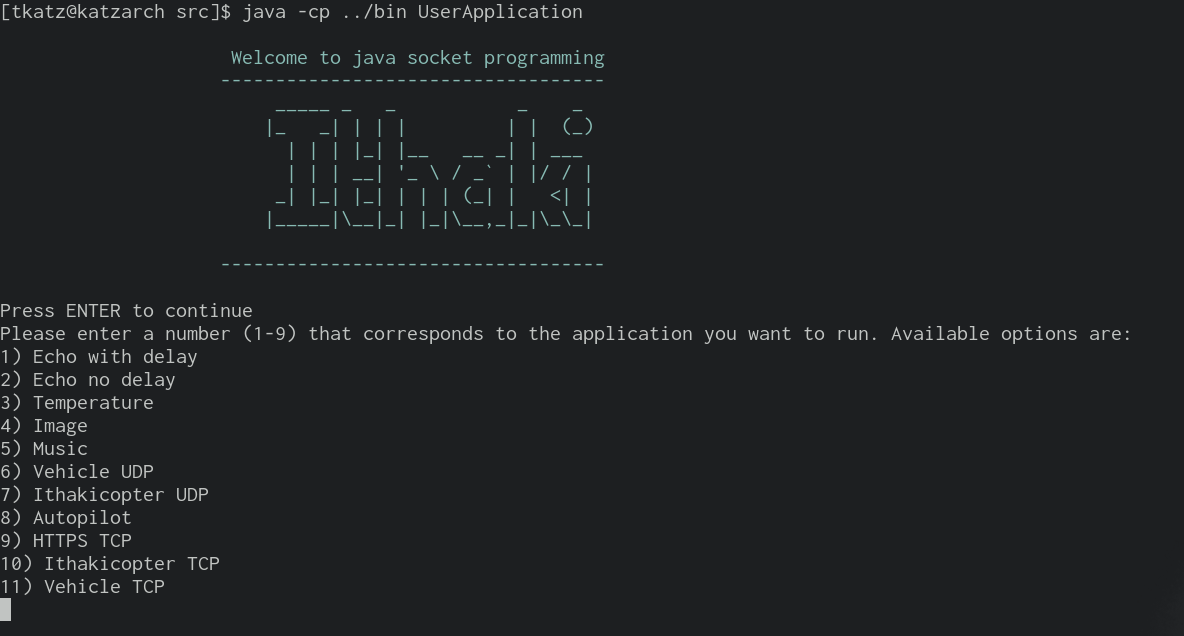
\includegraphics[width=\textwidth]{assets/login.png}}
% \author{Θεόδωρος Κατζάλης \\ ΑΕΜ:9282 \\ katzalis@auth.gr}
% \date{19/07/2020}

\begin{document}
\sloppy % this is legend

\begin{titlepage}

\begin{figure}[h!]
  \begin{center}
    
\includegraphics[width=3cm]{assets/auth.pdf}
    \label{fig:cover_auth_logo}
  \end{center}
\end{figure}

\centering
\Large Αριστοτέλειο Πανεπιστήμιο Θεσσαλονίκης\\
\Large Πολυτεχνική Σχολή\\
%\large Τμήμα Ηλεκτρολόγων Μηχανικών και Μηχανικών Υπολογιστών\\
%\large Τομέας Τηλεπικοινωνιών

\vspace{\fill}

\LARGE \textbf{Java socket programming} \\
\LARGE \textbf{Δίκτυα 2}

\vspace{\fill}

\Large Θεόδωρος Κατζάλης \\
\Large ΑΕΜ:9282 \\ 
\Large katzalis@auth.gr

\vspace{\fill}
\raggedright

\centering
\vspace{\fill}
\today

\end{titlepage}

%\maketitle


\pagebreak
\tableofcontents
\pagebreak

% \section{Lorem}
% \lipsum


\section{Εισαγωγή}

Η συγκεκριμένη εργασία αποσκοπεί στην εξοικείωση εννοιών σχετικά με τα δίκτυα υπολογιστών τόσο σε θεωρητικό όσο και σε πρακτικό επίπεδο. Αυτό εξασφαλίζεται με την δημιουργία δικτυακών εφαρμογών χρησιμοποιώντας την γλώσσα προγραμματισμού \textbf{java} σε συνεργασία με τον server ithaki του μαθήματος με IP 155.207.18.208. Αυτή λοιπόν η συνεργασία επιτρέπει \textbf{active} έλεγχο και καθορισμό ορισμένων παραμέτρων αλλά και \textbf{passive} συλλογή δεδομένων επειτα απο συγκεκριμένα request του χρήστη στον server. Προς το τελος αυτου του report θα γίνει αναφορά για πρωτόκολλα UDP και audio streaming.

Ενδεικτικά θα σημειώσουμε τις εφαρμογές που αναπτύχθηκαν με μια σύντομη περιγραφή τους. Η πλειοψηφία αυτών βασίζεται στο πρωτόκολλο UDP:
\begin{itemize}
    \item Echo.
        Αποστολή μηνύματος της μορφής ΕΧΧΧX και λήψη πακέτου με δεδομένα που αφορούν την τρέχουσα ημερομηνία και ώρα.
    \item Image.
        Αποστολή μηνύματος της μορφής ΜΧΧΧΧ και λήψη πακέτων που περιλαμβάνουν το byte content μιας φωτογραφίας jpg. The challenge: Βρες τους delimiters, την αρχή και το τέλος της εικόνας\footnote{Ακόμα και αν μια φωτογραφία jpg δεν έχει στο τελος του αρχείου σε δεκαεξαδική μορφή το ΟxFF D8, η φωτογραφία εξακολουθεί να απεικονίζεται σωστά}. 
    \item Audio.
        Αποστολή μηνύματος της μορφής ΑΧΧΧΧ και λήψη πακέτων ήχου κωδικοποιημένα σε DPCM και AQ-DPCM. The challenge: Κατανόσηση της κωδικοποίσης/αποκωδικοποίησης και βελτίωση της ποιότητασ του ήχου.
    \item Ithakicopter. Συλλογή τηλεμετρίας απο custom κατασκευή προσομοίωσης ελικοπτέρου. The challenge: Autopilot
    \item Car vehicle diagnostics. Συλλογή διαγνωστικών στοιχείων απο μια βάση δεδομένων σχετικά με κάποια στοιχεία λειτουργίας ενός αυτοκινήτου. The challenge: Υλοποίηση υπολογισμού δεδομένων και εισαγωγή στο πρωτόκολλο TCP και τα strams.
\end{itemize}


Όσον αφορά τα διαγράμματα που ακολουθούν, για λόγους πληρότητας, θα αναφέρουμε ότι τα ιστογράμματα έγιναν με την χρήση του λογισμικού στατιστικής SPSS και όλα τα υπόλοιπα διαγράμματα με  την χρήση της βιβλιοθήκης matplotlib της γλώσσας προγραμματισμού python! 

Ακόμη στα πλαίσια του \textbf{statement of originality}, έχουμε παραθέσει βιβλιογράφία για τις πηγές στις οποίες βασιστήκαμε για να φέρουμε εις περας αυτήν την εργασία. Στο κομμάτι του κώδικα, αρχικός κόμβος ερεθισμάτων αποτέλεσε η αναφορά του ίδιου του μαθήματος. Οπότε θα την παραθέσουμε και πρώτη\cite{ergasia2}.
\section{Session 1}


Σχετικά με την χρονοκαθυστέρηση και την ρυθμαπόδοση των echo packets έχουμε να αναφέρουμε τα εξής:

\subsection{Echo packets Delay: ON}

\subsubsection{Χρόνος απόκρισης}
\begin{itemize}
    \item Μέση τιμή: 1815 milliseconds και τυπική απόκλιση: 557 milliseconds
    \item Αρκετά υψηλή η δεύτερη σε σύκγριση με την πρώτη το οποίο υποδηλώνει ότι τα δείγματα μεταξύ τους δεν είναι "συμπυκνωμένα"και αποκλίνουν σημαντικό βαθμό απο την μέση τιμή.
    \item Δεν φαίνεται με ξεκάθαρο τρόπο ποια κατανομή ακολουθούν τα δεδομένα μας, ωστόσο με κάποια επιφύλαξη θα μπορούσαμε να ισχυριστούμε ότι ακολουθούν bimodal κατανομή. Αυτό το συμπέρασμα προέκυψε απο την τάση να σχηματιστούν δύο καμπάνες.
\end{itemize}

\subsubsection{Ρυθμαπόδοση}

\begin{itemize}
    \item Μέση τιμή: 109 bits/sec και τυπική απόκλιση: 30.04 bits/sec
    \item Ομοίως με την μελέτη της χρονικής απόκρισης, η τυπική απόκλιση είναι αρκετά υψηλή, περίπου το 30\% της μέσης τιμής
    \item Σχετικά με την κατανομή θα μπορούσαμε να υποστηρίξουμε ότι ακολουθεί right skewed normal distribution.
\end{itemize}
Παρατηρώντας το διάγραμμα της \textbf{ρυθμαπόδοσης} (throughput) διακρίνουμε ότι το εύρος τιμών κυμαίνεται περίπου απο 70 μέχρι 180 bits/second. Αξίζει να σημειωθούν κάποιες σχεδιαστικές αποφάσεις οι οποίες λήφθηκαν κατα τη διάρκεια υλοποίησης του αλγορίθμου της ρυθμαπόδοσης:

Σύμφωνα με την περιγραφή της άσκησης, ο υπολογισμός έπρεπε να γίνει με την τεχνική του κινούμενου μέσου όρου. Επιλέξαμε τα 8 δευτερόλεπτα ως το χρονικό πλαίσιο λήψης δεδομένων για κάθε δείγμα ρυθμαπόδοσης το οποίο υπολογίζεται για κάθε δευτερόλεπτο σε μήκος 4 συνεχόμενων λεπτών λήψης echo packets. Συνεπώς για τα τελευταία 8 δευτερόλεπτα απο τα 4 λεπτά της συνολικής μέτρησης δεν έχουν υπολογιστεί δείγματα ρυθμαπόδοσης. 

Η ύπαρξη των spikes στο διάγραμμα ερμηνεύεται απο το αν πρόλαβε κάποιο πακέτο στο πλαίσιο των 8 δευτερολέπτων να συμπεριληφθεί στο ένα δείγμα και όχι στο άλλο. Για παράδειγμα, αν έρθει ένα πακέτο την χρονική στιγμή $t_1 = t + 6.5$ second, και το επόμενο έρθει την χρονική στιγμή $t_2 = t + 8.1$, τότε το δείγμα της ρυθμαπόδοσης που μετρόυσε απο $[t, t+8]$ δεν θα λάβει υπόψιν το πακέτο που έφτασε στα $t + 8.1$. Ωστόσο στο δείγμα της ρυθμαπόδοσης που ξεκινάει απο $[t+8, t+16]$ θα συμπερλιγθεί η τιμή του. Συγκεκριμένα, η τιμή αυτή είναι $32*8$ bits, αφού το κάθε echo packet response περιέχει 32 bytes\footnote{Ο τρόπος με τονο οποίο διαπιστώσαμε το μέγεθος των δεδομένων έγινε με την βοήθεια του wireshark} δεδομένα. Για αυτό μπορούμε να παρατηρήσουμε ότι τα spikes διαφέρουν απο τα υπόλοιπα δείγματα πολλαπλάσια του $32$.


\subsection{Echo packets Delay: OFF}

\subsubsection{Χροόνος απόκρισης}
Στην συγκεκριμένη περίπτωση η χρονοκαθυστέρηση των δειγμάτων μειώνεται αισθητά σε χαμηλότερες τιμές milliseconds με αποτέλεσμα να λαμβάνουμε αρκετά περισσότερα δείγματα συγκριτικά με την προηγούμενη περίπτωση. Συνεπώς για λόγους ευκρίνειας (engineering appreciation όπως έχει ειπωθεί και στο μάθημα) παραθέυτουμε μια zoom in εκδοχή του διαγράμματος του χρόνου απόκρίσης με εύρος ενδεικτικά απο 100-200 packets. Σε γενικές γραμμές το εύρος της χρονοκαθυστέρησης κυμαίνεται απο 230-260 milliseconds. Πιο συγκεκριμένα έχουμε:
\begin{itemize}
    \item Μέση τιμή: 237 milliseconds και τυπική απόκλιση: 7 milliseconds 
    \item Συγκριτικά με Delay: ON, βλέπουμε ότι η τυπική απόκλιση είναι αρκετά μικρή σε σχέση με την μέση τιμή, επομένως τα δείγματα δεν έχουν την τάση να είναι "αραιωμένα".
    \item Σχετικά με την κατανομή μπορούμε να διακρίνουμε την δημιουργία δύο στενών καμπανών γύρω απο τις τιμές 232 και 246. Συνεπώς θα μπορούσμα να ισχυριστούμε για μια ακόμη φορά bimodal distribution. 
\end{itemize}

\subsubsection{Ρυθμαπόδοση}
Για τις σχεδιαστικές αποφάσεις καθως και την ερμηνεία των spikes, έχει γίνει ήδη αναφορά στην προηγούμενη ανάλυση (Delay: ON).

Όπως έχει αναφερθεί, ο αριθμός των πακέτων που φτάνουν στον δέκτη είναι πολύ μεγαλύτερος με μικρότερη χρονοκαθυστέρηση μεταξύ των πακέτων, συνεπώς η ρυθμαπόδοση αυξάνεται αισθητά.
\begin{itemize}
    \item Μέση τιμή: 1040 bits/sec και τυπική απόκλιση: 18 bits/sec.
    \item Εξίσου μικρή η τυπική απόκλιση συγκριτικά με την μεση τιμή.
    \item Σχετικά με τη κατανομή μιας και οι τιμές συγκεντρώνεται στο αριστερό κομμάτι του γραγήματος θα μπορούσαμε να υποθέσουμε λογαριθμική κατανομή.
\end{itemize}


'Οσα έχουνα αναφερθεί μέχρι στιγμής αφορούν τον σχολιασμό των διαγραμμάτων G1-G8.

\subsection{Retransmission timeout (RTO)}


Για λόγους γρήγορης και αξιόπιστης επικοινωνίας σχετικά με το πρωτόκολλο TCP, υπάρχει η ανάγκη πρόβλεψης και επαναπροσδιόρισης των παραμέτρων timeout σε ένα σύστημα επικοινωνίας. Πόσο πρέπει να περιμένει ο sender αν δεν λάβει  ACK απο τον receiver για να ξαναστείλω την πληροφορία; Ο προσδιορισμός των timers είναι λοιπόν πολύ σημαντικός διότι αν δεν ρυθμιστεί σωστά, υπάρχει η πιθανότητα να ξανααστένουμε πακέτα πολύ γρήγορα προτού ο δέκτης να προλάνει να στείλει ACΚ ή το ανάποδο, δηλαδή να περιένουμε πολύ να ξαναστείλουμε ένα πακέτο\cite{gfg_rto, saminir}. 

Υπάρχουν κάποιες μαθηματικές σχέσεις οι οποίες υπολογίζουν τον retransmssion timer και υπάρχουν συγκεκριμένα 3 σταθερές α, β και γ. Εμείς επιλέξαμε αρχικά σταθερά τα α και β με τιμές $1 - 1/8 = 0.875$ και $1 - 1/4 = 0.750$. Επίτηδες γράψαμε με αυτήν την μορφή της εξισώσεις προκειμένου να είμαστε συμβατοί με το notation των εξισώσεων που μας δίνονται στο πλαίσιο μαθήματος, μιας και οι αναφορές\cite{rfc}, τα δικα μας α και β, τα συμβολίζουν ως (1-α) και (1-β). Για την επιλογή του γ (k σύμφωνα με RFC) δοκιμάσαμε στην αρχή την προτεινόμενη τιμή 4. Στη συνέχεια παρατηρώντας το γράφημα R1 προσπαθούσαμε να φτάσουμε την γραμμή RTO να αγκαλιάζει το RTT, δηλαδή να μην είναι πολύ πάνω αλλά και ούτε απο κάτω του RTT. Τελικά επιλέξαμε την τιμή 1,8 και βλέπουμε ότι ικανοποητικά η γραμή RTO ακολουθεί σωστά το RTT.

\subsection{Tone frequency}

Γνωρίζουμε ότι η εικονική γεννήτρια συχνοτήτων παράγει δύο ημίτονα και στέλνει την πληροφορία με κωδικοποίσησ DPCM. Χρησιμοποιώντας το εργαλείο audacity, προκειμένου να βρούμε τις συχνότητες, στο πρώτο session, παρατηρώντας τα spikes του spectrum plot, μπορούμε να εικάσουμε επιλέγοντας τις υψηλότερες κορυφές, ότι οι συχνότητες των ημιτόνων είναι 421 και 343 Hz.

\begin{figure}[h!]
\centering
	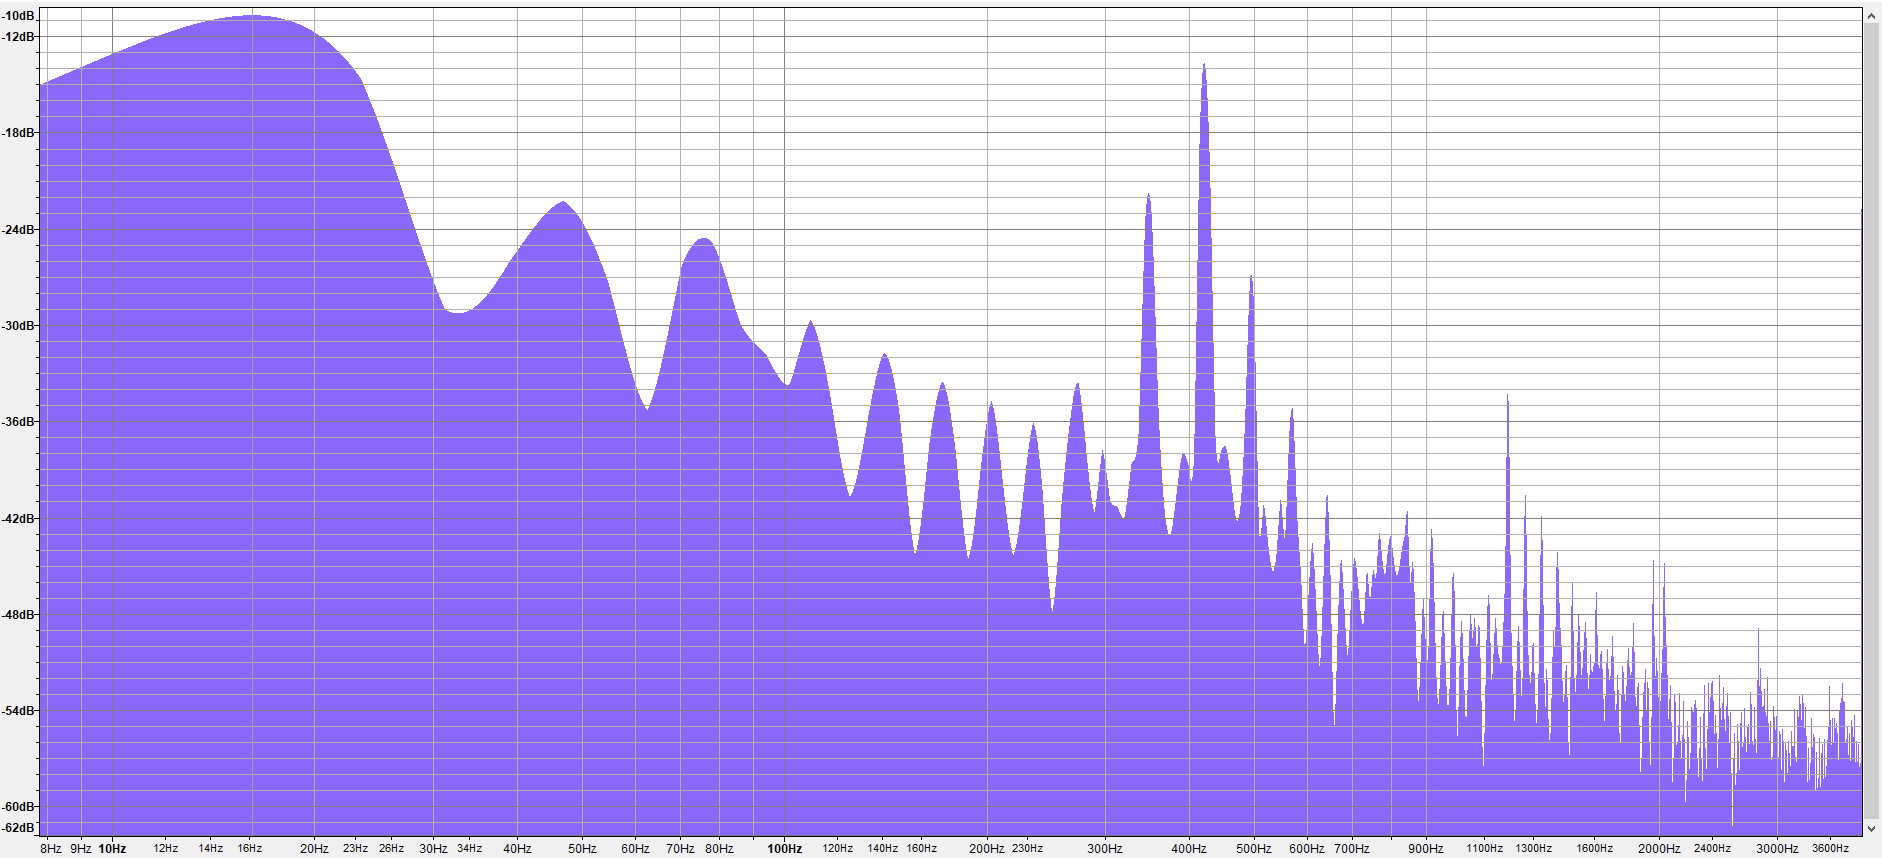
\includegraphics[height=.3\textheight, width=\textwidth]{assets/session1/spectrum.png}
    \caption{Frequency spectrum}
\end{figure}

\subsection{Image}

Κατά τη διάρκεια ανάπτυξης της εφαρμογής της εικόνας. στην προσπάθεια μας να δημιουργήσουμε real-time video, αλλάξαμε το μέγεθος των πακέτων απο 128 σε 1024 χρησιμοποιώντας το κατάλληλο request code και καταφέραμε λαμβάνοντας 100 δείγματα να δημιουργήσουμε ένα βίντεο 40 δευτερολέπτων κάνοντας merge τα δείγματα αυτά. Το video μπορείτε να το δείτε \href{https://drive.google.com/file/d/1yfwckvGBr8YteigF3ainMJMXwLOzjZ9u/view?usp=sharing}{εδώ}. Αξίζει να σημειωθεί οτι για το βίντεο χρησιμοποιήσαμε την κάμερα FIX. Θα μπορούσαμε να χρησιμοποιούσαμε την PTZ για να είχαμε πιο πιστευτή πραγματική αναπαράσταση μιας και ο χρόνος λήψης της εικόνας είναι πιο μικρός εξαιτίας της μικρότερης ανάλυσης της.

Σχετικά με τον χρόνο που αποτυπώνουν οι εικόνες, παρατηρήσαμε οτι στην FIX η ημερομηνία και η ώρα είναι ακριβής, ενώ στην PTZ υπάρχει μια καθυστέρηση της τάξης των 4 λεπτών περίπου. Φυσικά με κατάλληλες εντολές DIR=X, υπάρχει και η δυνατότητα απεικόνισης του πύργου του ΟΤΕ (session 2).

\subsection{Audio}

Σχετικά με τον ήχο χρησιμοποιήσαμε τους κωδικούς L22 και L11 για τα ζητούμενα της εργασίας: 
\begin{itemize}
    \item L22:
    \item L11: 
\end{itemize}

Όσον αφορά τα γραφήματα του ήχου μπορούμε να παρατηρήσουμε το λεγόμενο \textbf{clipping effect}. Εξαιτίας της αναδρομικής σχέσης στην αποκωδικοποίηση DPCM και AQ-DPCM για την λήψη των πραγματικών δειγμάτων, υπάρχει περίπτωση οι τιμές των samples να υπερβούν τις μέγιστες και τις ελάχιστες των 8 και 16 bits που χρησιμοποιήθηκαν για την κβάντιση τους. Οπότε προκειμένου να αποφύγουμε το ενδεχόμενο να γίνει roll back απο την μεγαλύτερη τιμή στην μικρότερη, κάθε φορά που ο integer (32 bits) ξεπερνούσε την μεγιστη τιμή ή την ελάχιστη τιμή των bits κωδικοποίσης, τότε το θέταμε ίσο με το μέγιστο ή το ελάχιστο αντίστοιχα. Για αυτό το λόγο επίσης μπορουε να ερμηνεύσουμε και στο ιστόφραμμα, ιδιαίτερα υψηλές τιμές στις ελάχιστες όπου γινόταν το clipping.

Επειδή ο αριθμός των δειγμάτων είναι ιδιαίτερα υψηλός, έχουμε προσθέσει στα διαγράμματα ήχου και zoom in εκδοχές προκειμένου να έχουμε μια αίσθηση του τρόπου διακύμανσης των τιμών σε τοπικό επίπεδο. Ενδιαφέρον παρουσιάζει το διάγραμμα του τόνου, απο την εικονική γεννήτρια συχνοτήτων, στο οποίο μπορούμε να παρατηρήσουμε το σχηματισμό ενός ημιτονοειδούς σήματος!

Σχετικά με την μέση τιμή, η οποία προστίθεται στα δείγματα, έχει μικρή τιμή συγκριτικά με τις διαφορές των δειγμάτων οι οποίες καθορίζονται σε μεγάλο βαθμό απο τις μεγάλες τιμές του step.

Το request code audio που φαίνεται στο wireshark αντιστοιχίζεται στην κυματομορφή AQ-DPCM (G9), ενώ τα υπόλοιπα δείγματα έχουν ληφθεί για το ίδιο τραγούδι αλλά διαφορετικές χρονικές στιγμές.

\subsubsection{AQ-DPCM}

\begin{itemize}
    \item Το ιστόγραμμα των διαφορών των δειγμάτων για AQ-DPCM δείχνει μια τριγωνική/κανονική κατανομή και ένα απότομο spike. Οι τιμές των δειγμάτων έχουν υψηλές τιμές της τάξης των χιλιάδων με μέση τιμή -48 και τυπική απόκλιση κοντά στα 4000.
    \item Το ιστόγραμμα των ίδιων των σημάτων φαίνεται να ακολουθεί κανονική κατανομή right skewed με μέση τιμή -11600 και τυπική απόκλιση 10282. Το clipping effect συμβάλει στο spike του ιστογράμματος, καθώς πολλές τιμές που υπερβαίνουν τα όρια συγκεντρώνεται σε εκείνη την περιοχή, την ελάχιστη τιμή των 16 bits προσημασμένου ακεραίου.
\end{itemize}


\subsubsection{DPCM}

Το DPCM απο την άλλη πλευρά μας δείχει δύο πολύ καθαρά γραφήματα όσον αφορά τις διαφορές των δειγμάτων και των ίδιων των δειγμάτων. Τα δεδομένα και στις δύο περιπτώσεις φαίνεται να ακολουθούν τριγωνική κατανομή. Αξίζει να σημειωθεί οτι οι τιμές είναι αρκετά πιο χαμηλές σε σύγκριση με το AQ-DPCM, μιας και θεωρούμε ότι το step είναι ίσο με 1, σε αντίθεση με το AQ στο οποίο μας έρχεται ως πληροφορία το step και έχει και ιδιαίτερα υψηλές τιμές επηρεάζοντας σημαντικά τις διαφορές των δειγμάτων.


\subsection{Ithakicopter and car diagnostics}


\section{Section 2}


\subsection{Audio}

Audio clips L01 and L02

\section{Tone frequency}

Μια αρκετά πιο καθαρή εικόνα σε σύκγριση με το plot spectrum στο session 1. Με παρόμοια λογική βλέποντας τις κορυφές των τριγώνων εικάζουμε ότι οι συχνότητες ειναι 1024 και 349 Hz.

\begin{figure}[h!]
\centering
	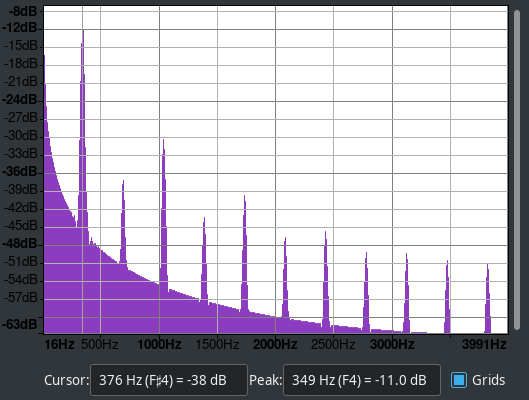
\includegraphics[height=.3\textheight, width=\textwidth]{assets/session2/spectrum.png}
    \caption{Frequency spectrum, 1042 Hz and 349 Hz}
\end{figure}


\section{Ανάλυση πηγαίου κώδικα}
\subsection{Image}
Μπορεί να γίνει αναφορά ότι η υπαρξη θορύβου εξαιτίας κβάντισης και καναλιού μπορεί να οδηγήσει στην αλλοιώση των delimiters με αποτέλεσμα ο να μην επιτυχής η εύρεση τους. Η υλοποίσηση μας ωστόσο προσπαθεί να βρει καθώς έρχονται τα πακετα τον delimiter. Σε περίπτωση που αποτύχει, τότε θα δεχτεί timeout, θα εκτελεστεί το catch block και θα συνεχίσει η ροή του προγράμματος.

\subsection{RTO}
'Εχει γίνει ήδη αναφορά για το πως βρήκαμε τις σταθερές και τον αλγόριθμο.

\subsection{User Interface}

\begin{figure}[h!]
\centering
	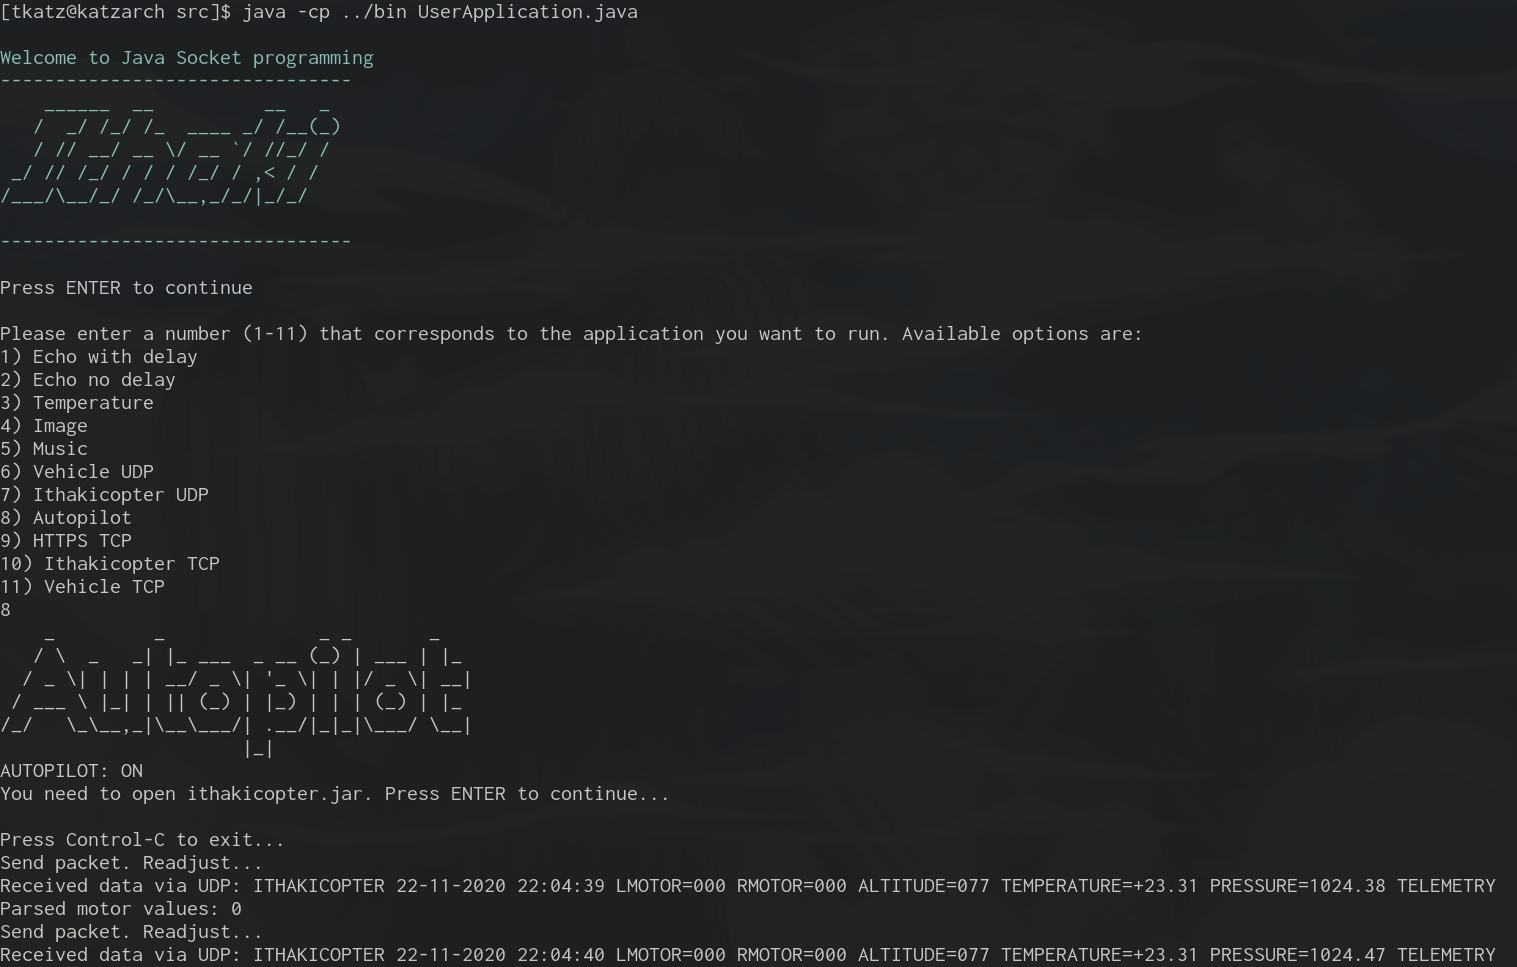
\includegraphics[width=\textwidth]{assets/ui.png}
	\caption{Εκτέλεση προγράμματος σε κέλυφος Bash} 
    \label{fig:ui}
\end{figure}




\section{UDP}
Here we are going to talk about UDP protocol.



\section{Audio streaming protocols}




\clearpage

\bibliographystyle{plain}
\bibliography{bib/bib.bib}

\end{document}
